


\begin{figure}[htbp]
    \centering
    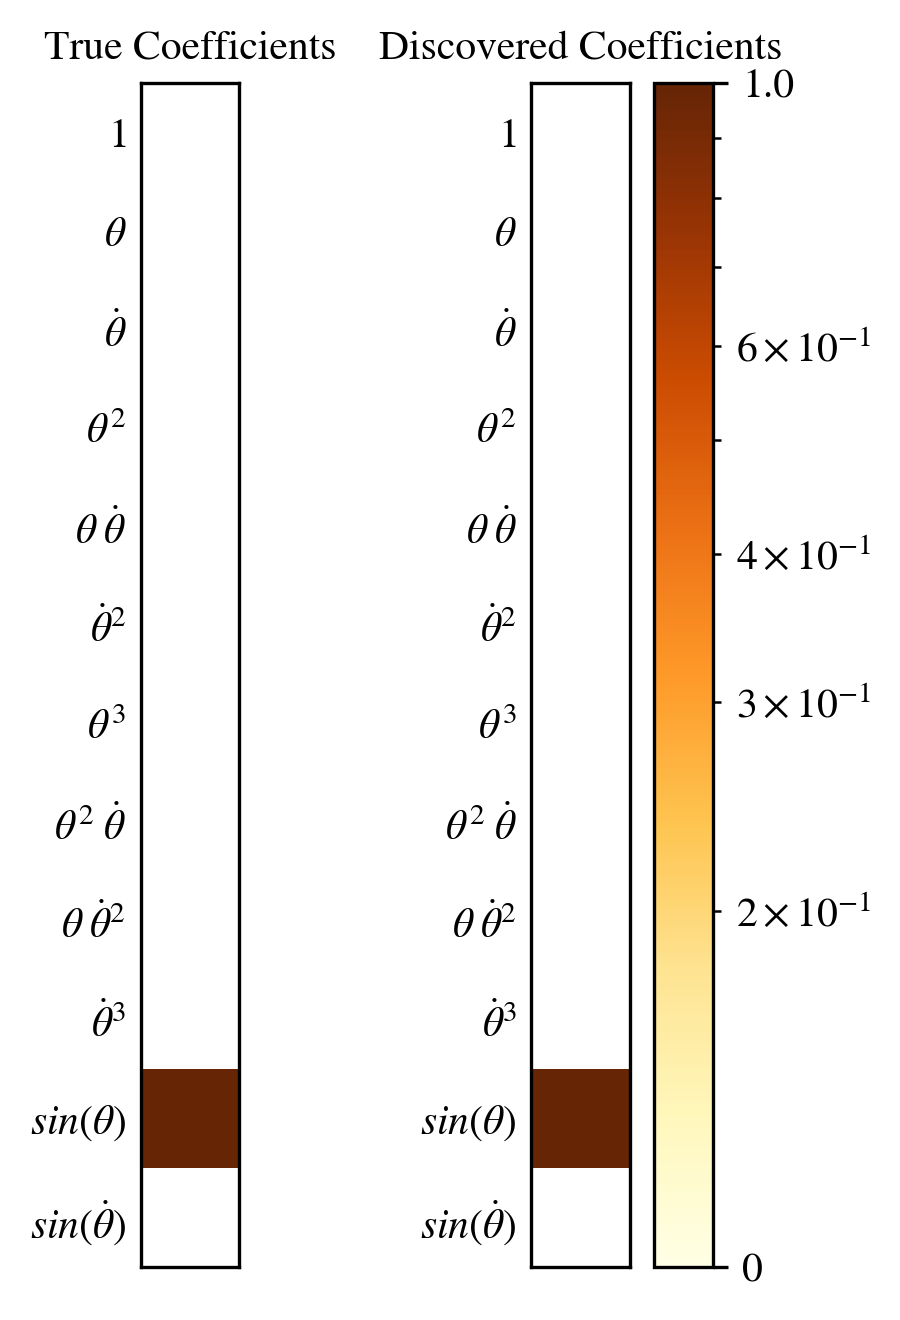
\includegraphics[width=0.43\textwidth]{project_2/images/xi_plot_pendulum.png}
    \vspace{-3mm}
    \caption{\textbf{Comparison of True and Discovered Coefficients for Pendulum Dynamics:} This figure juxtaposes the exact coefficients (left) against those identified by the modeling framework (right) for various dynamical terms of the pendulum, ranging from linear terms like $\theta$ and $\dot{\theta}$ to nonlinear interactions such as $\theta^2\dot{\theta}$ and trigonometric functions like $\sin(\theta)$. Each coefficient's magnitude is represented by the color intensity, with the scale shown on the right. The perfect alignment in coefficient values demonstrates that the discovered model is exactly identical to the true model, confirming the framework's precision in capturing the complete dynamics of the pendulum system.}
    \label{fig:xi_plot_pendulum}
\end{figure}

\begin{figure*}[t]
\centering
\begin{minipage}[b]{.45\textwidth}
\centering
   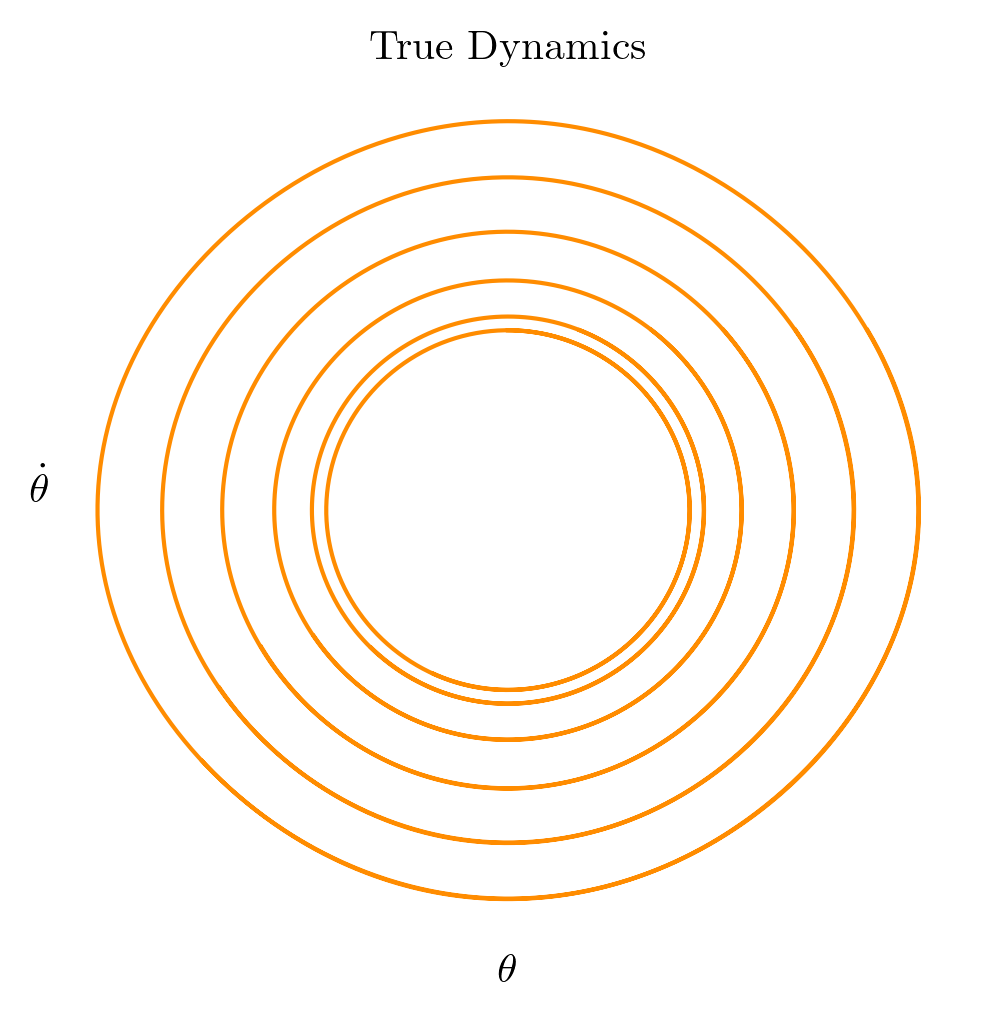
\includegraphics[width=\textwidth]{project_2/images/z_zdot_true.png}
   \vspace{-3mm}
    \caption{\textbf{True pendulum phase space:} This figure shows the phase portrait of a true pendulum system. The diagram depicts the trajectories in the $\theta$-$\dot{\theta}$ phase space under gravitational forces. Each loop represents the motion of the pendulum at a different energy level, with the innermost loop corresponding to the smallest amplitude of oscillation.}
    \label{fig:true_z_zdot_pendulum}
\end{minipage}\qquad\quad
\begin{minipage}[b]{.45\textwidth}
\centering
    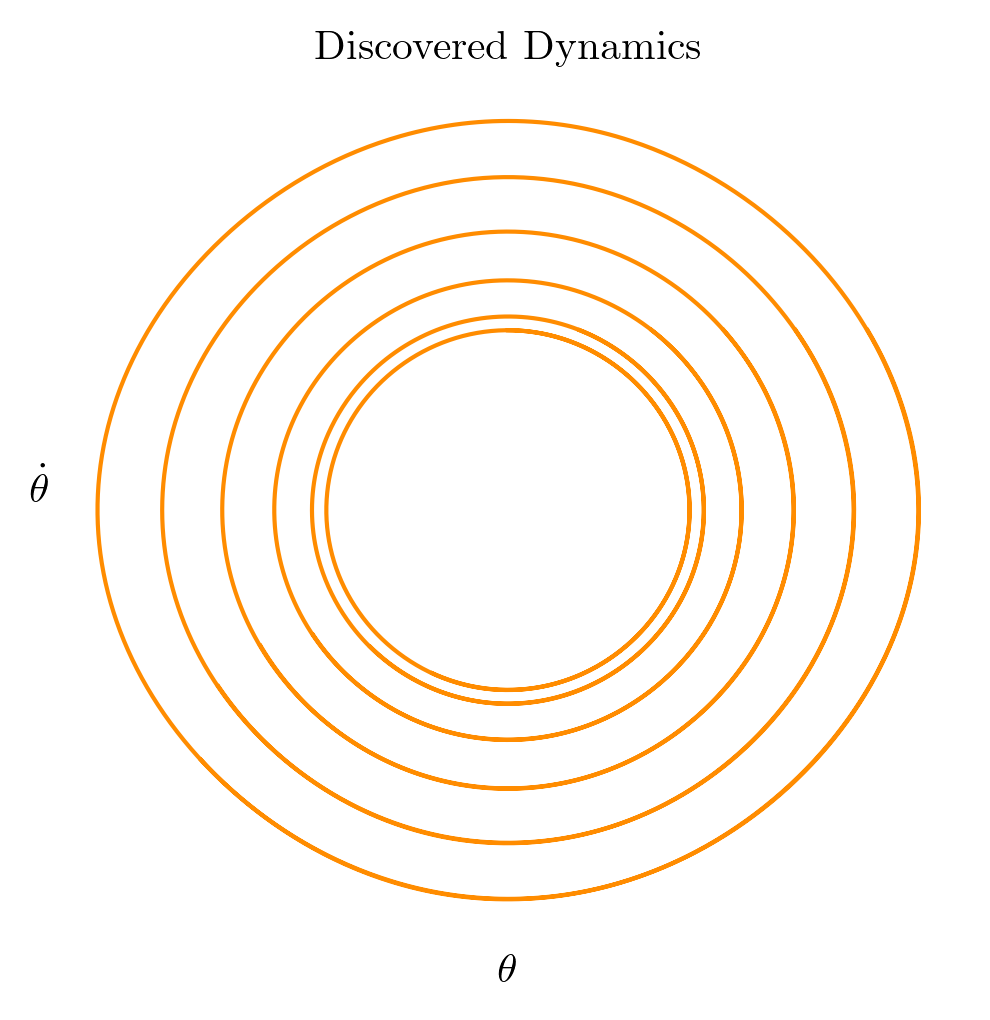
\includegraphics[width=\textwidth]{project_2/images/z_zdot_discovered.png}
    \vspace{-3mm}
    \caption{\textbf{Discovered Pendulum Phase Space:} This figure shows the phase portrait of the pendulum dynamics discovered by the autoencoder SINDy framework, depicted in the $\theta$-$\dot{\theta}$ phase space. The estimated trajectories closely mirror those of the true dynamics, exhibiting consistent structural features across all energy levels as illustrated in \autoref{fig:true_z_zdot_pendulum}.}
    \label{fig:discovered_z_zdot_pendulum}
\end{minipage}
\end{figure*}

% \begin{figure}[htbp]
%     \centering
%     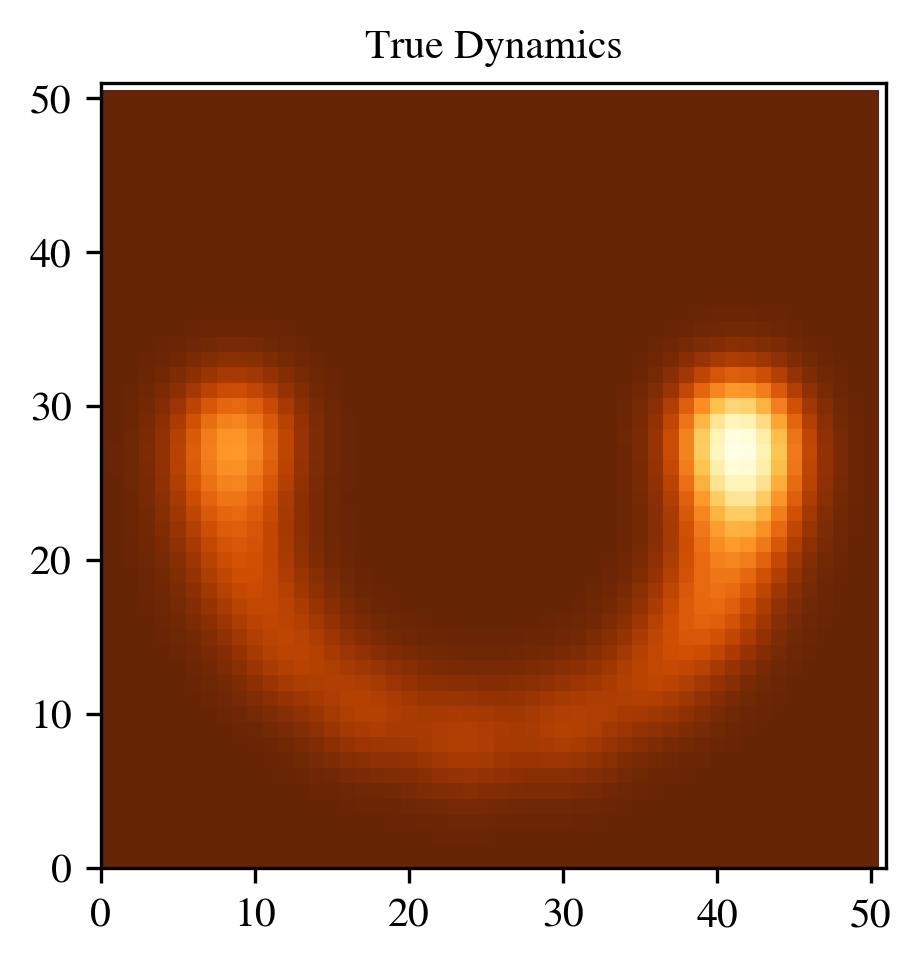
\includegraphics[width=0.43\textwidth]{project_2/images/true_heatmap_pendulum.png}
%     \caption{}
%     \label{fig:true_heatmap_pendulum}
% \end{figure}

% \begin{figure}[htbp]
%     \centering
%     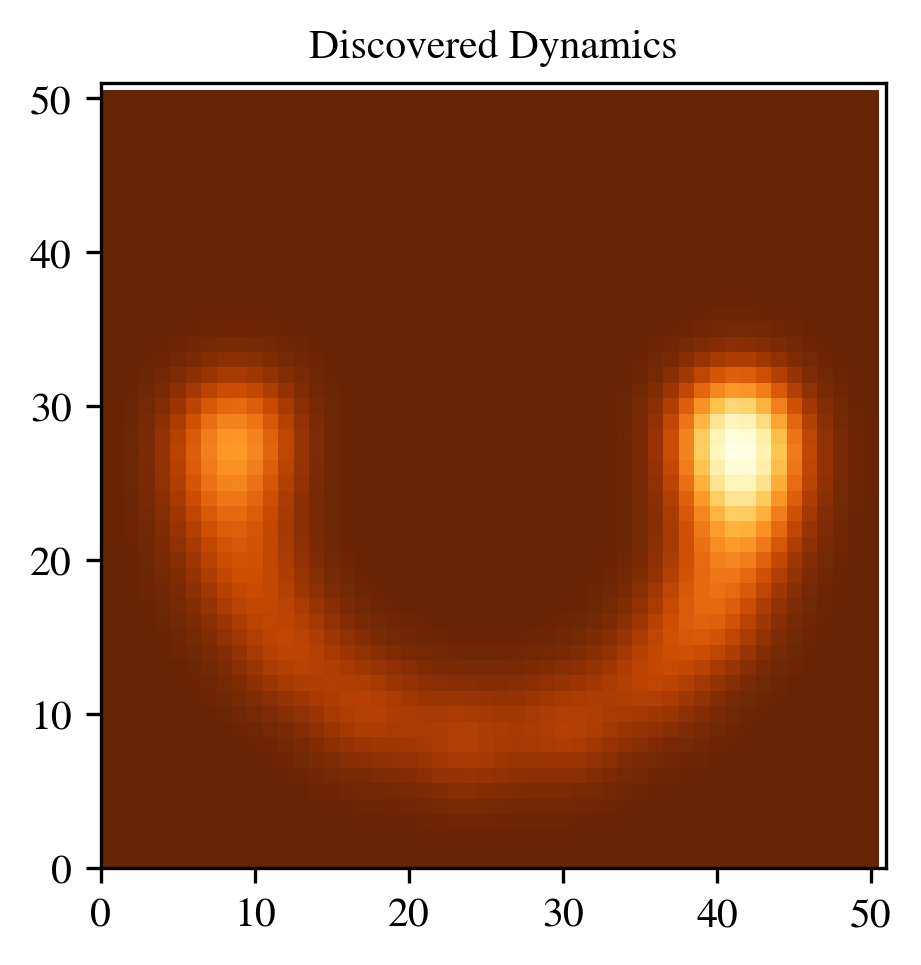
\includegraphics[width=0.43\textwidth]{project_2/images/discovered_heatmap_pendulum.png}
%     \caption{}
%     \label{fig:discovered_heatmap_pendulum}
% \end{figure}

